\documentclass{article}
\usepackage[a4paper, portrait, margin=1in]{geometry}
\usepackage{tabularx}
\usepackage{graphicx}
\usepackage{amsmath}
\usepackage{amsfonts}
\usepackage{algorithm}
\usepackage[noend]{algpseudocode}


\title{AIW \& Information Retrieval (UE18CS322)\\Unit 1}
\author{Aronya Baksy}
\date{January 2021}

\begin{document}

\maketitle

\section{Introduction}
\begin{itemize}
    \item Information Retrieval can be defined as finding material (documents) of an unstructured nature (usually text), that satisfies a given information need from within large collections (often stored on computers)
    
    \item Scope of IR:
    \begin{itemize}
        \item Most text on the internet is semi-structured, meaning that even though the English language itself has no overt structure (other than the inherent semantics of the language), the vast majority of text is organized into documents, headings, sub-headings, paragraphs etc.
        
        \item Clustering documents together based on the similarity of their contents
        
        \item Classification based on topic, or other classes (such as age range, other information needs)
    \end{itemize}
        
    \item IR systems operate at various scales:
    \begin{itemize}
        \item \textbf{Web search}: Involving billions of documents on millions of machines, efficient and fast indexing, exploiting hyperlinks and avoiding manipulation of page content by sites to boost hits
        
        \item \textbf{Personal IR}: Programs such as email search, or search utilities in consumer OSes like MacOS Spotlight Search and Windows Cortana Search, must be efficient and lightweight to be able to run on a single PC.
        
        \item \textbf{Enterprise, Institutional, domain-based search}: restricted domain search, larger than personal but smaller than global web search. 
    \end{itemize}
\end{itemize}

\section{Boolean Information Retrieval}
\begin{itemize}
    \item A Boolean IR Model is one that can answer any query that involves a set of terms combined by Boolean operators (\textit{AND}, \textit{OR}, \textit{NOT})
    
    \item One basic strategy for handling of Boolean queries is to use a pattern-matching program (eg: \texttt{grep} available on *nix systems) to iteratively scan through each document to see which documents satisfy the given query.
    
    \item The disadvantages of this approach are:
    \begin{itemize}
        \item For large-scale corpora like the set of all documents on the WWW, this is a time consuming task
        
        \item It does not allow for non-Boolean queries, or they may be impractical to do (eg: get all documents where Caesar and Calpurnia are at most 5 words apart)
        
        \item It does not allow for ranked retrieval, i.e. to decide which of the retrieved results is the "best" based on some measure of goodness.
    \end{itemize}
    
    \item An \textit{information need} is a topic or some information that the user wishes to know more about. This information need is expressed to the computer (the IR system) in the form of a \textit{query}.
    
    \item A result of a query is considered to be \textit{relevant} if the user perceives it as containing value with respect to their information need. 
    
    \item The effectiveness of an IR system is measured in terms of Precision and Recall
\end{itemize}

\subsection{Basic Index construction}
\begin{itemize}
    \item The most basic form of term-document indexing is called the incidence matrix $C$. The rows of the matrix correspond to the terms, and the columns correspond to the documents in the collection.
    
    \item For a term $t_i$ and a document $d_j$
    \begin{equation*}
        C(t_i, d_j) = \begin{cases}
        1 \text{ if term $t_i \in$ document $d_j$} \\
        0 \text{ if term $t_i \notin$  document $d_j$}
        \end{cases}
    \end{equation*}
    
    \item Any Boolean query can then be answered by taking the incidence vectors for each term (i.e. the corresponding row of the matrix $C$) and then applying the corresponding Boolean operations in a bit-wise fashion. 
    
    \item The term-document matrix is a sparse matrix (i.e. the majority of entries in it are 0) hence storing the entire matrix in memory is not feasible 
    
    \item This model ignores information about term frequency within a document and positional information of terms within a document. 
\end{itemize}

\subsection{Inverted Index construction}
\begin{itemize}

    \item The inverted index is called so because the search query asks for documents, but the index consists of terms that point to documents (or document IDs), i.e. the index is build by term and not directly by document.
    
    \item The inverted index consists of 2 parts: a \textit{dictionary} of terms and a list of \textit{postings}
    
    \item Vocabulary is defined as the \textbf{set} of all unique terms across the corpus
    
    \item The dictionary is a data structure that stores each term of the vocabulary, along with a pointer to its posting list (which is stored on disk) and additional info about that term (e.g. the number of documents it appears in, called the \textit{document frequency})
    
    \item A posting list for a particular term $t$ is a list of document IDs that the term $t$ appears in. For later convenience the posting list is maintained in sorted order by document ID.
    
    \item Steps involved in Inverted index construction are as follows:
    \begin{enumerate}
        \item Tokenization of documents into tokens
        
        \item Normalization of tokens. This involves processes like conversion to a single uniform case (typically lowercase), lemmatization and stemming which are carried out by NLP modules (like \texttt{nltk} in Python, \texttt{stringr} in R). 
        
        \item Generate a sequence of $\langle$ term, docID $\rangle$ pairs for each normalized term in each document. Sort this sequence, first in lexical order of term, and then by docID.
        
        \item Merge multiple entries for a single term into a single posting list. The length of this posting list is the document frequency (number of documents in which that term appears). 
        
        \item Separate the dictionary component (term, document frequency and pointer to posting list. stored in memory) and posting list component (stored on disk).
    \end{enumerate}
    
    \item To resolve Boolean queries of the form $x\text{ }AND\text{ }y$ we use the \textit{intersect} algorithm to find the intersection of the posting lists of terms $x$ and $y$.
    
    \item The intersect algorithm works in linear time $O(|x| + |y|)$ where $|x|$ and $|y|$ are the lengths of the two posting lists. 
    
    \item A slight modification of the intersect algorithm results in the union algorithm that works in linear time, to produce the union of two posting lists

\end{itemize}

\begin{figure}[!t]
    \centering
    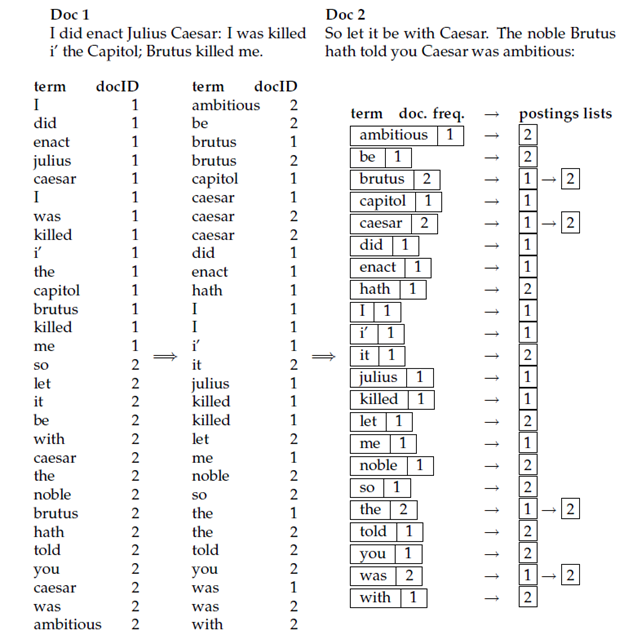
\includegraphics[scale=0.9]{ir.png}
    \caption{Example for Inverted Index construction}
    \label{fig:my_label}
\end{figure}

\begin{algorithm}
\caption{Intersect Algorithm}
\begin{algorithmic}
    \Procedure{intersect}{$p_1$, $p_2$}
    \State $answer \leftarrow \langle \rangle$
    \While{$p_1 \not= NULL$ and $p_2 \not= NULL$}
        \If{docID($p_1$) = docID($p_2$)}
            \State ADD(answer, docID($p_1$))
            \State $p_1 \leftarrow$ next($p_1)$
            \State $p_2 \leftarrow$ next($p_2)$
        \ElsIf{docID($p_1$) $<$ docID($p_2$)}
            \State $p_1 \leftarrow$ next($p_1)$
        \Else 
            \State $p_2 \leftarrow$ next($p_2)$
        \EndIf
    \EndWhile
    \Return answer
    \EndProcedure
\end{algorithmic}
\end{algorithm}

\begin{algorithm}
\caption{Union Algorithm}
\begin{algorithmic}
    \Procedure{union}{$p_1$, $p_2$}
    \State $answer \leftarrow \langle \rangle$
    \While{$p_1 \not= NULL$ and $p_2 \not= NULL$}
        \If{docID($p_1$) = docID($p_2$)}
            \State ADD(answer, docID($p_1$))
            \State $p_1 \leftarrow$ next($p_1)$
            \State $p_2 \leftarrow$ next($p_2)$
        \ElsIf{docID($p_1$) $<$ docID($p_2$)}
            \State ADD(answer, docID($p_1$))
            \State $p_1 \leftarrow$ next($p_1)$
        \Else 
            \State ADD(answer, docID($p_2$))
            \State $p_2 \leftarrow$ next($p_2)$
        \EndIf
    \EndWhile
    
    \If{$p_1 < len(p_1)$}    \Comment{Add remaining entries from list 1 if any}
        \While{$p_1 < len(p_1)$}    
            \State ADD(answer,  docID($p_1$))
            \State $p_1 \leftarrow$ next($p_1)$
        \EndWhile
    \EndIf
    \If{$p_2 < len(p_2)$}  \Comment{Add remaining entries from list 2 if any}
        \While{$p_2 < len(p_2)$}    
            \State ADD(answer,  docID($p_2$))
            \State $p_2 \leftarrow$ next($p_2)$
        \EndWhile
    \EndIf
    \Return answer
    \EndProcedure
\end{algorithmic}
\end{algorithm}

\begin{itemize}
    \item The NOT operation may or may not be completed in linear time.
    
    \item The strengths of a Boolean query model are that it is precise and it is simple to implement. 
    
    \item The weaknesses of a Boolean query model are:
    \begin{itemize}
        \item Not tolerant to spelling mistakes
        
        \item Cannot handle phrase search as it does not store any position information for each term within a document. 
        
        \item Does not give importance to term frequency within a document
        
        \item Does not retrieve documents in ranked order of relevance
    \end{itemize}
\end{itemize}

\subsection{Case Study on Boolean Retrieval: Westlaw}
\begin{itemize}
    \item Westlaw is an IR system for legal research that supports enhanced Boolean querying over tens of TBs of legal data stored as text
    
    \item Apart from the above discussed Boolean operators, Westlaw also implements other operators such as the \textbf{proximity operator} (a method of specifying that 2 terms must appear near each other in a document, nearness is defined as either number of words in between or in terms of grammar structures like paragraphs or sentences)
    
    \item Some operators used in the Westlaw IR system are:
    \begin{itemize}
        \item \textbf{!}: A wildcard operator, represents zero or more characters (eg: access! represents all words starting with the prefix "access" such as accessed, accessing, accessory etc. 
        
        \item \textbf{/p}: Represents that two terms must appear in the same paragraph 
        
        \item \textbf{/s}: Represents that two terms must appear in the same sentence. 
        
        \item Whitespace: Represents the OR operator (disjunction)
        
        \item \textbf{/n} where $n$ is an integer: represents that two terms must appear within $n$ words of one another
    \end{itemize}
    
    \item e.g.: \textbf{disabl! /p access! /s work-place work-site (employment /3 place)} means the words with prefix "disabl" appearing in the same paragraph as words with prefix "access" appearing the same sentence as either the word "work-place" or the word "work-site" or the phrase having "employment" at 3 words distance from "place"
\end{itemize}

\subsection{Boolean Query Optimization}
\begin{itemize}
    \item For queries that consist of conjunction (AND) of $n$ terms, the queries can be processed in increasing order of size.
    
    \item The AND operation that yields the \textit{smallest possible set} as its answer is done first (as the size of the result is then constrained to this size). For this reason the document frequency (i.e. length of individual posting lists) is stored in the dictionary
    
    \item For queries involving OR of 2 terms, the formula 
    \begin{equation*}
       | A \cup B |  = |A| + |B| - |A \cap B|
    \end{equation*}
    can be used. Since the value of $|A \cap B|$ is not known, a conservative estimate of the union size is 
    \begin{equation*}
       | A \cup B | \approx |A| + |B|
    \end{equation*}
    
    \item Using this estimate, the union queries can be processed in increasing order of size (smallest first). 
\end{itemize}

\section{Words, Tokens and Terms}
\subsection{Tokenization}
\begin{itemize}
    \item A token is defined as an instance of a sequence of characters 
    in a particular document that are grouped together as a single semantic useful unit for processing.
    
    \item A type is the class of all tokens containing the same sequence of characters. A token is the (maybe normalized) type that is included in the dictionary of the IR system. 
    
    \item Tokenization is the process of splitting up a block of text into tokens.
\end{itemize}
\subsubsection{Issues with Tokenization}
\begin{itemize}
    \item Handling words with \textbf{apostrophes} in them. e.g.: "Finland's Capital" could be tokenized as either $\langle$ Finland, s, Capital $\rangle$ or $\langle$ Finlands, Capital $\rangle$. This issue also occurs in languages like French. 
    
    \item \textbf{Domain-specific} tokens. e.g.: Aircraft names like B-52, A-320 or F-16, programming languages like C++ and C\#, TV shows like F.R.I.E.N.D.S, IP addresses, web URLs, package tracking numbers. Such tokens are normally removed from the vocabulary to keep the dictionary size reasonable, but certain meta-data items like creation dates etc. can be indexed separately. 
    
    \item \textbf{Hyphenation} is used in English for various purposes (separating vowels lke co-education, joining nouns like Hewlett-Packard, or word groupings like three-hundred-year-old trees). Splitting such words into tokens is either handled as a classification problem, or other heuristic rules.
    
    \item Splitting tokens with \textbf{whitespaces} in them (e.g.: Los Angeles which is a single token but white space split would make it into two). Splitting on whitespace can cause bad results as well (e.g.: a query for York University might yield documents containing New York University). 
    
    \item \textbf{Language specific} issues. For example, compound nouns in German are not split by space, e.g. lebensversicherungsgesellschaftsangestellter means life insurance company employee. Or the fact that Chinese text is never split by white space, or that Arabic/Hebrew are written from right to left except sequences like numbers that are read left to right. 
\end{itemize}

\subsection{Stop word Removal}
\begin{itemize}
    \item Stop words are extremely common tokens which do not contain any semantic information that enhances the meaning of a sentence/paragraph. 
    
    \item Examples of stop words are a, an, and, are, is, the, for, from
    
    \item Stop words can be identified by sorting terms by their collection frequency (number of times a term appears in the entire document collection), picking the $k$ most frequently occurring terms and then hand-filtering those terms by their semantic content. The list of terms with little or no semantic content can be dropped from the index. 
    
    \item Removal of stop words generally does no harm to performance of IR systems while reducing memory requirements, but phrase search will be affected by stop word removal (e.g.: a query for the phrase "to be or not to be")
    
    \item General trend in IR systems is reduction in size of stop lists (currently very few IR systems use stop lists, web search engines do not use them). 
\end{itemize}

\subsection{Normalization (equivalence classing of terms)}
\begin{itemize}
    \item Normalization is the processes of converting all tokens into a canonical form such that two or more sequences can match despite having superficial differences between one another. 
    
    \item Most common method of normalization is implicitly creating equivalence classes using mapping rules (e.g.: deleting hyphens or deleting periods) to match tokens to a common form (e.g.: anti-discriminatory and antidiscriminatory can be mapped to the same class, so do U.S.A and USA).
    
    \item Relations between un-normalized tokens can be maintained using an index of un-normalized tokens each of which lead to an expansion list of vocabulary terms to consider for that given query term (hence a query term is an AND of the posting lists for all the corresponding synonym index terms)
    
    \item The above can also be done during the construction of the index. (e.g.: if "automobile" is encountered in a document that docID can be added to both "automobile" and "car" posting lists)
\end{itemize}

\subsubsection{Techniques for Normalization}
\begin{itemize}
    \item \textbf{Accents and diacritics} are generally removed due to issues with rendering them and the fact that they are less frequently used in queries (even though some words carry different meanings with and without a single accent)
    
    \item \textbf{Case-folding}, i.e. the conversion of all characters to a uniform case , most often lower case. This allows resolution of more queries but causes problems between common nouns and proper nouns (eg: General Motors)
    
    \item \textbf{True casing}: Using machine learning sequence models, or simple heuristic rules to normalize the case. (rules may be like: all uppercase words in a title or at the start of a sentence can be made lowercase, but all other uppercase words retain their original case). 
    
    \item Using heuristics for normalizing words in foreign languages that may have different spellings and conventions. Most often used is the \textbf{Soundex algorithm} that classes terms with similar phonetic sounds together. Also used heuristic is the \textbf{edit distance}. 
\end{itemize}

\subsection{Lemmatization and Stemming}
\begin{itemize}
    \item Reducing all inflectional and variant forms of a word to a common base form is the goal of both stemming and lemmatization.
    
    \item Stemming uses a crude heuristic that involves chopping off the ends of words in the hope of achieving this normalization (direct removal of derivative suffixes)
    
    \item Lemmatization refers to the use of a vocabulary and morphological analysis of words, normally aiming to remove inflectional endings only and to return the lemma (base form of the word). 
    
    \item Most common stemming algorithm is the \textbf{Porter Stemmer}. It is a\textbf{ fast rule based approach} that uses 5 sequential steps: the first step involves a rule-based direct replacement, and the following steps use the \textit{measure} of the word (\# of syllables) to detect whether a suffix is derivative or is actually a part of the word
    
    \item Other stemming algorithms are \textbf{Snowball Stemmer} and the \textbf{Paice-Husk Stemmer}. 
\end{itemize}

\section{Inverted Index Optimization}

\subsection{Intersection Algorithm with Skip pointers}

\begin{algorithm}
\caption{Intersect Algorithm with Skip Pointers}
\begin{algorithmic}
    \Procedure{intersect\_skip}{$p_1$, $p_2$}
    \State $answer \leftarrow \langle \rangle$
    \While{$p_1 \not= NULL$ and $p_2 \not= NULL$}
        \If{docID($p_1$) = docID($p_2$)}
            \State ADD(answer, docID($p_1$))
            \State $p_1 \leftarrow$ next($p_1)$
            \State $p_2 \leftarrow$ next($p_2)$
        \ElsIf{docID($p_1$) $<$ docID($p_2$)}
            \If{hasSkip($p_1$) \textbf{and} (docID(skip($p_1$)) $\leq$ docID($p_2$))}
                \While{hasSkip($p_1$) \textbf{and} (docID(skip($p_1$)) $\leq$ docID(p2))}
                    \State $p_1$ $\leftarrow$ skip($p_1$)
                \EndWhile
                \State $p_1 \leftarrow$ next($p_1)$
            \ElsIf{hasSkip($p_2$) \textbf{and} (docID(skip($p_2$)) $\leq$ docID($p_1$))}
                \While{hasSkip($p_2$) \textbf{and} (docID(skip($p_2$)) $\leq$ docID($p_1$))}
                    \State $p_2$ $\leftarrow$ skip($p_2$)
                \EndWhile
                \State $p_2 \leftarrow$ next($p_2)$
            \EndIf
        \EndIf
    \EndWhile
    \Return answer
    \EndProcedure
\end{algorithmic}
\end{algorithm}
\begin{itemize}
    \item The presence of skip pointers (i.e. pointers that allow one to skip multiple entries in a list rather than traverse in the linked order only) allows for faster traversal and eliminates docIDs that will not feature in the final result faster.
    
    \item The placing of skips involves a trade-off between large skip length (fewer pointer comparisons but also fewer chances to skip) and large number of skip pointers with short length (more likely to skip but more space needed to store pointers and also more pointer comparisons)
    
    \item A simple heuristic for pointer placement is, in a list of length $P$, there should be $\sqrt{P}$ evenly-spaced skip pointers. 
    
    \item Skip pointers are useful for static document collections, but do not work with dynamic document collections. 
\end{itemize}

\subsection{Positional Indices}
\begin{itemize}
    \item Different approaches are needed to support phrase queries (i.e. queries composed of more than one term such as "Stanford university")
\end{itemize}

\subsubsection{Bi-Word Indices}
\begin{itemize}
    \item In a bi-word index, each pair of consecutive terms is considered as a single dictionary entry. Such pairs are referred to as bi-words
    
    \item e.g.: The phrase "friends, Romans, countrymen" yields the bi-words "friends Romans" and "Romans countrymen". 
    
    \item Multi-word queries (more than 2 words) can be broken up into bi-word pairs and then the intersection of all the intermediate results gives the answer. 
    
    \item This can result in \textit{false positives} when the result contains all the pairs but not consecutively. These have to be resolved using hand-filtering.
    
    \item Queries that consists of linking grammar structures such as "abolition of slavery" and "cost overruns on a power plant" can be resolved using Parts-Of-Speech Tagging (POS Tagging)
    
    \item Phrases of the form N x* N where N represents a noun and x represents any other word can be considered as \textbf{extended bi-words}. The extended bi-words can also be added to the index in order to resolve queries of the above form. 
    
    \item Drawbacks of bi-word indexes are
    \begin{itemize}
        \item Tendency to result in false positives
        
        \item Size of the index blows up due to larger vocabulary size
    \end{itemize}
    
    \item However some bi-word queries (such as "Narendra Modi" or "Joe Biden") are very popular in web IR systems hence they can be included as part of the index. 
\end{itemize}

\subsubsection{Positional Indices}
\begin{itemize}
    \item In a positional index, a posting list for a term consists not only of the docID where it appears, but also a list of positions in that document where that term appears
    
    \item e.g.: $\langle$ term, doc freq $\rangle$: $\langle$ $\langle doc_1$: $p_1, p_2, p_3$ $\rangle$, $\langle doc_2$: $p_1, p_2, p_3$ $\rangle$ $\rangle$
    
    \item To evaluate queries of the form "University of Minnesota":
    \begin{itemize}
        \item The posting lists of "University" and "Minnesota" are retrieved
        
        \item The common doc IDs are found using the intersect algorithm
        
        \item For each doc ID in the intersection set, the condition is checked whether Minnesota appears at a gap of 1 word after University. The doc IDs that satisfy the condition are returned. 
    \end{itemize}
    
    \item The above step can be extended to any length of gap between 2 terms in a phrase query (such as /n proximity queries in Westlaw IR)
    
    \item Positional indices are substantially larger than normal inverted indices, but the extra storage is offset by the larger flexibility and usefulness. 
    
    \item In a \textbf{combination scheme}, frequent bi-words are indexed normally as vocabulary terms, but the remaining terms are stored as positional indices. 
    \item The choice of which bi-words to store is based on how often these bi-words are queried for, and what is the time saving if they were directly stored in a bi-word index. 
\end{itemize}

\subsection{Posting List Implementation}
\begin{itemize}
    \item Fixed size array posting list leads to large amounts of wasted space. Variable sized arrays address this issue.
    
    \item Arrays work well for static corpora (where the action on the list is mostly read, hence due to caching based on locality of reference, accesses become faster)
    
    \item Dynamic indices are best implemented as linked lists, despite the extra space needed to store pointers, as insertion and deletion in linked lists can be done in constant time in linked list. 
    
    \item For large posting lists, using linked list is not a good idea as it leads to large number of disk seeks during traversal (large list does not fit in memory). Arrays make more sense in this case.
\end{itemize}

\subsection{Dictionary Implementation}
\begin{itemize}
    \item Most often used data structures are hash table and Binary Search Tree (or its balanced and more general version, the B-Tree).
\end{itemize}
\subsubsection{Hash Table}
\begin{itemize}
    
    \item In a hash table, the term is converted to an integer by the \textit{hash function}. This integer is used to access the relevant term information (the doc frequency and the pointer to posting list) from the table
    
    \item At query time: first find the index using hash function, then resolve collision (i.e. multiple terms having same hash value) and then locate the correct entry.
    
    \item \textbf{Pros}: Hash table has lookup time complexity of $O(1)$ (constant time)
    
    \item \textbf{Cons}: 
    \begin{itemize}
        \item Minor variants of a single query term may not be close to each other in the hash table
        
        \item No prefix search
        
        \item For dynamic corpora, rehashing is needed to avoid large number of collisions
    \end{itemize}
\end{itemize}

\subsubsection{Binary Search Tree}
\begin{itemize}
    \item BST is a type of tree wherein all keys in the left sub-tree of a node are smaller and all keys in the right sub-tree are larger in value than the key at that node.
    
    \item \textbf{Pros}: 
    \begin{itemize}
        \item Allow prefix queries
        
        \item Terms are always stored in sorted order
    \end{itemize}
    
    \item \textbf{Cons}:
    \begin{itemize}
        \item Insertion takes more time than hash table($O(log N)$ time complexity only for balanced trees, this degrades to $O(N)$ for unbalanced trees)
        
        \item Rebalancing a BST to keep the height optimal is an expensive operation
    \end{itemize}
\end{itemize}

\subsubsection{B Trees}
\begin{itemize}
    \item Every internal node has number of children in the range $[a, b]$ where $a<b$ and $a, b \in \mathbb{Z}^+$
    
    \item B-trees allow for prefix search like BST but also solve the issue of balancing
    
    \item A large $b$ results in a fatter and shorter tree
\end{itemize}

\section{Tolerant Retrieval}
\subsection{Wildcard Queries}
\begin{itemize}
    \item The wildcard character * represents any sequence of 0 or more characters. Any query with * in it can be considered as a wildcard query
    
    \item Queries where the * appears at the end are called prefix queries (e.g.: "mon*" signifies all words that start with the prefix "mon"). As seen before a B-Tree based index easily handles prefix queries
    
    \item Queries with * at the beginning are called suffix queries (e.g.: "*mon" gives all words ending with mon). To service such queries, another inverted index of \textbf{reversed terms} is stored. The reverse index is accessed for such queries.
    
    \item Queries of the form X*Y where X and Y are sequences of characters are resolved as follows:
    \begin{itemize}
        \item Retrieve terms that contain X* from the normal B Tree
        
        \item Retrieve terms that contain *Y from the reversed B Tree
        
        \item Intersect these two term lists. 
        
        \item Find the OR (disjunction) of all the posting lists of the terms in this intersection. 
    \end{itemize}
    
    \item For more complicated queries, the process involves multiple uses of the intersect algorithm which is an expensive operation. The \textbf{permuterm index} is used in such a scenario
\end{itemize}

\subsection{Permuterm Index}
\begin{itemize}
    \item For every term in the standard inverted index, add a special character \$ to the end, and rotate the term about the \$ character. The \$ indicates the end of a string
    
    \item All the possible rotations of a word are indexed to that word in an index called the permuterm index. 
        
    \item e.g.: For hello\$ the rotations are ello\$h, llo\$he, lo\$hel, o\$hell. All these rotations are indexed to the same word "hello" in the permuterm index. 
    
    \item For wildcard queries of the form m*n\$, it can be transformed into n\$m*. From the permuterm index, the terms that match this query can be extracted and the standard inverted index can be queried to get the documents.
    
    \item For wildcard queries of the form x*y*z\$, look up z\$x* first from the permuterm index. This gives us a list of terms that satisfy the query x*z. Now from these, filter out the terms that contain y in them. 
    
    \item Permuterm index is an efficient method for allowing wildcard queries, but its dictionary takes up a large amount of space due the number of rotations of a term that need to be stored for all terms. 
\end{itemize}

\subsubsection{K-gram Index}
\label{kgram}
\begin{itemize}
    \item The special \$ character is used here to denote the beginning or the end of a term. 
    
    \item In a k-gram index, the dictionary contains all k-grams that appear in the corpus. Each k-gram points to a posting list of terms that contain that k-gram. 
    
    \item These lists are sorted in lexicographical order so as to allow the intersect algorithm to run.
    
    \item e.g.: for the term \$castle\$, the possible 3-grams are \$ca, cas, stl, tle, le\$. Hence the term "castle" would appear in the posting lists for all five of these 3-grams. 
    
    \item Assuming a 3-gram index, given a query like re*ve, the 3-grams \$re and ve\$ are searched, and the intersection of the two term lists is found. 
    
    \item Given the same 3-gram index and a query like red*, the 3-grams to be searched are \$re and red. This leads to false positives like the term "retired" which satisfies both \$re and red but does not satisfy the original query.
    
    \item To avoid these false positives, the intersection list is filtered by hand to check whether the terms match the original query. This is done using a simple string match. 
    
    \item Most search engines and other IR systems hide the wildcard query functionality behind some "Advanced Search" option, as it is an expensive operation to process such queries, and also because such queries are rarely used in practice. 
\end{itemize}

\subsection{Spelling Correction}
\begin{itemize}
    \item Spelling correction can either be used to correct misspelled words within the corpus, or to correct misspelled words in the query.
    
    \item Document error correction is used for documents retrieved using OCR using tuned algorithms and domain knowledge. 
    
    \item For query correction, either the original query is itself modified to the correct one and documents are retrieved, or the system suggests corrections that the user can choose from, which can be used by the system. 
    
    \item In \textbf{isolated} spelling correction, each word is corrected on its own, without considering the neighbouring words in the phrase. This approach does not catch typos caused by correctly spelled words (e.g.: I ducking hate this course)
    
    \item In \textbf{context-sensitive} spelling correction, the decision to correct an error is taken based on the surrounding words. 
\end{itemize}

\subsubsection{Edit Distance}
\begin{itemize}
    \item For isolated spelling correction, a notion of similarity between 2 words is needed. The edit distance is one such measure
    
    \item The edit distance between two strings $s$ and $d$ is the least number of transformations (insert character anywhere, delete any character, change a single character) needed to transform $s$ into $d$. 
    
    \item Dynamic programming can be used as the edit distance computation has the overlapping sub-problems property. Assume a memoization matrix $D$ that stores the edit distance. Arrange the letters of source $s$ along the vertical and letters of destination $d$ along the horiziontal
    
    \item Then the matrix is filled using:
    \begin{equation*}
        D(i, j) = min \begin{cases}
            D(i-1, j) + 1 \\
            D(i, j-1) + 1 \\
            D(i-1, j-1) + \begin{cases}
                1 \text{ if s(i) $\neq$ d(j)}\\
                0 \text{ if s(i) $=$ d(j)}\\
            \end{cases}
    \end{cases}
    \end{equation*}
    
    \item Then the bottom right entry of the matrix is the minimum edit distance
    
    \item Maintaining back-pointers as the optimal operation is chosen at each step allows the optimum path to also be known
    
    \item The weighted edit distance captures the weight of an operation (insert, delete, update) as per the characters involved in that operation (e.g.: m is more likely to be mistyped as n than as q, hence m-n distance is smaller)
    
    \item The modified recurrence relation is now:
    \begin{equation*}
        D(i, j) = min \begin{cases}
            D(i-1, j) + del(s(i)) \\
            D(i, j-1) + ins(d(j)) \\
            D(i-1, j-1) + \begin{cases}
                subs(s(i), d(j)) \text{ if s(i) $\neq$ d(j)}\\
                0 \text{ if s(i) $=$ d(j)}\\
            \end{cases}
    \end{cases}
    \end{equation*}
    
    \item The edit distance can be used for query correction in the following manner:
    \begin{itemize}
        \item \textbf{Approach 1}: Generate all character sequences that are at edit distance $d$ from the query. Intersect this list with the correct words set in the dictionary. Show the terms to the user as suggestions for the user to act
        
        \item \textbf{Approach 2}: IR system looks up all possible corrections and returns the relevant documents. This can be refined by considering a single most likely correction (using the collection frequency of the corrected terms). 
    \end{itemize}
\end{itemize}

\subsubsection{k-gram Index}
\begin{itemize}
    \item Using the k-gram index (refer \ref{kgram}) spelling correction can be refined further. 
    
    \item Given the set of all k-grams in the query term, the term lists for each k-gram can be retrieved from the k-gram index. 
    
    \item The naive approach is to compute the set of all terms that contain atleast $n$ of the k-grams that are present in the query. (e.g.: for a query "bord" the 2-grams are bo, or, rd. The terms that contain at least 2 of the 3 k-grams may be "boardroom", "aboard", "border")
    
    \item This naive approach fails to give appropriate corrections ("boardroom" for "bord"). Hence a more nuanced measure of similarity is needed. 
    
    \item The \textbf{Jaccard similarity} between 2 sets $X$ and $Y$ is defined as
    \begin{equation}
        sim_J(X, Y) = \frac{|X \cap Y|}{|X \cup Y|}
    \end{equation}
    
    \item A single linear scan through the entire vocabulary is done. For each vocabulary term $t$ the Jaccard similarity is computed with the query term $q$.
    
    \item If $sim_J(q, t) > sim_{min}$ where $sim_{min}$ is some minimum threshold for the similarity, then $t$ is added to the list of possible corrections. 
    
    \item note: computation of Jaccard similarity only needs lengths of 2 strings, hence it is efficient to do on the fly. 
\end{itemize}

\subsubsection{Context-Sensitive Spelling Correction}
\begin{itemize}
    \item Given a query with $n$ words, take one word at a time, find its possible corrections and substitute them in the query.
    
    \item Run each substituted query by the IR system and see which query gives the largest number of results. 
    
    \item This approach is costly if each term contains a large number of corrections possible. Several heuristics are used to trim this space, sich as hit-based refinement
    
    \item Hit-based refinement is used to optimize this to a certain extent:
    \begin{itemize}
        \item Hits in corpus: number of times the suggested query appears in corpus
        
        \item Hits in query logs: number of times a suggested query appears in past queries done by users. 
    \end{itemize}
    
    \item Bi-word based spelling correction is a technique where the query is first split into list of bi-words, then the bi-words that are common (again based on the hit-based refinement) are chosen to be expanded. 
\end{itemize}

\subsubsection{Phonetic Spelling Correction}
\begin{itemize}
    \item The Soundex algorithm (invented in 1918 for the US Census) is used for this purpose. 
    
    \item Each term in the vocabulary is converted into a 4-character long code. Convert the query into a code and then retrieve all terms with the same code. 
    
    \item The algorithm is summarized as follows:
    \begin{itemize}
        \item Retain the first letter of the term
        
        \item Replace all occurrences of A, E, I, O, U, H W, Y with 0
        
        \item Substitute letters with numbers according to the rule:
        \begin{itemize}
            \item B, F, P, V $\rightarrow$ 1
            \item C, G, J, K, Q, S, X, Z $\rightarrow$ 2
            \item D, T $\rightarrow$ 3
            \item L $\rightarrow$ 4
            \item M, N $\rightarrow$ 5
            \item R $\rightarrow$ 6
        \end{itemize}
        
        \item Replace all pairs of consecutive digits with one digit
        
        \item Remove all 0s from the string. Pad the remaining places with 0 and return the first 4 characters of the result. It should be of the form letter followed by 3 digits.
        
        \item e.g.: HERMANN becomes H655, HERMAN becomes H655 too
    \end{itemize}
    
    \item Soundex is implemented in many RDBMS (MS SQL Server, Oracle, PostgreSQL, etc.). It is not very useful for terms that are not names, and it has been shown to be biased towards certain nationalities. 
    
    \item Soundex is suited for high recall tasks but may not offer good precision.
\end{itemize}
\end{document}
